\documentclass[12pt]{article}

\title{Real dimension in the Newtonian simulation of disk-like pressure-free systems}
\author{S. Halayka\footnote{sjhalayka@gmail.com}}
\date{\today\;\currenttime}

\usepackage{datetime}
\usepackage{listings}
\usepackage{cite}
\usepackage{xcolor}
\usepackage{graphicx}
\usepackage{setspace}
\usepackage{amsmath}
\usepackage{url}
\usepackage[margin=0.8in]{geometry}
\usepackage{listings}


\usepackage{xcolor}
\lstset { %
    language=C++,
    backgroundcolor=\color{black!5}, % set backgroundcolor
    basicstyle=\footnotesize,% basic font setting
    showstringspaces=false,
}


%\doublespace

%\usepackage[]{lineno}
%\linenumbers


\begin{document}



 
\maketitle

\begin{abstract}
Newtonian gravitation is given in terms of gravitational field lines.
C++ code is provided.
\end{abstract}




\section{Entropy}
Entropy is a measure of how much information is required to encode a particular macroscopic state.
For example, in terms of the set of 8-bit integers, where there are $W$ distinct microstates, the binary entropy $n$ is:
\begin{equation}
n = \frac{\log W}{\log 2}.
\end{equation}
The number of distinct 8-bit integers is 256, and so the binary entropy is 8 and W is 256.

At low density (e.g. everyday densities on the Earth), this binary entropy is proportional to mass.

At the highest density (e.g. black hole densities), this binary entropy is proportional to mass squared.
For instance, using binary entropy:
\begin{equation}
n = \frac{A_s k c^3}{ 4 G \hbar \log 2},
\end{equation}

It was 't Hooft's idea to quantize the black hole's event horizon area into gravitational field line emitters in his pioneering work on the holographic principle.




\section{Brute force: field line intersection density gradient}

In this paper, we numerically solve for the Newtonian (e.g. Keplerian) and flat (e.g. constant velocity) gradients using a unit axis-aligned bounding box by obtaining the lengths of the intersecting line segments emitted by the gravitating body. See Fig.1. 



\begin{figure} 
\centering
\label{fig1}
  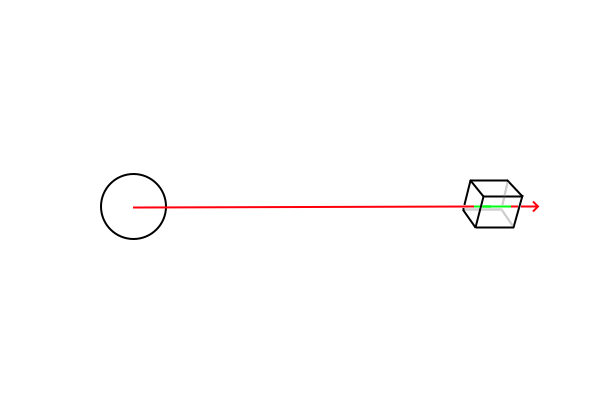
\includegraphics[width = 6 in]{AABB.png}
  \caption{
Where $D = 3$.
This figure shows a unit axis-aligned bounding box and an isotropic emitter, looking from above.
An example field line (red) and intersecting line segment (green) is given.
The bounding box is filled with these intersecting line segments.
It is the gradient of the density of these line segments that forms the gravitational acceleration.
}
\end{figure}





Regarding the holographic principle, the Schwarzschild black hole event horizon radius is:
\begin{equation}
r_s = \sqrt{\frac{A_s}{4 \pi}} = \sqrt{\frac{n G \hbar \log 2}{k c^3 \pi}},
\end{equation}
and the mass is:
\begin{equation}
M = \frac{c^2 r_s}{2 G} = \sqrt{\frac{n c \hbar \log 2}{4 G k \pi}}. 
\end{equation}

Where $R$ is some far distance from the centre of the gravitating body (e.g, $R \gg r_s$), $\beta$ is the get intersecting line length density function, and $\epsilon$ is some small value (e.g $10^{-5}$), the gradient (e.g. derivative) is:
\begin{equation}
\gamma = \frac{\beta(R + \epsilon) - \beta(R)}{\epsilon}.
\end{equation}
The gradient strength is:
\begin{equation}
g = -\gamma \pi = \frac{n}{2 R^3}.
\end{equation}
The Newtonian acceleration $a_{\textit{Newton}}$ is:
\begin{equation}
a_{\textit{Newton}} = \frac{v_{\textit{Newton}}^2}{R} = \sqrt{\frac{g G c \hbar \log 2}{2 R^2 k \pi}}.
\end{equation}

The acceleration $a_{\textit{flat}}$ for a flat rotation curve is:
\begin{equation}
a_{\textit{flat}} = \frac{v_{\textit{flat}}^2}{R} = \frac{g R c \hbar \log 2}{2 k \pi M}.
\end{equation}

The ratio of the two accelerations is
\begin{equation}
\frac{a_{\textit{flat}}}{a_{\textit{Newton}}} = R^{d}, 
\end{equation}
where $d = 3 - D$ stands for disk-like, and the dimension of the gravitation field is:
\begin{equation}
D = 3 - \frac{\log \frac{a_{\textit{flat}}}{a_{\textit{Newton}}}}{\log R} = 3 - \frac{\log \frac{v_{\textit{flat}}^2}{v_{\textit{Newton}}^2}}{\log R}.
\end{equation}

The following code shows how to calculate the field lines based on a disk-like emitter:
\begin{lstlisting}

bool intersect_AABB(
	const vector_3 min_location, 
	const vector_3 max_location, 
	const vector_3 ray_origin, 
	const vector_3 ray_dir, 
	double &tmin, double &tmax)
{
	 tmin = (min_location.x - ray_origin.x) / ray_dir.x;
	 tmax = (max_location.x - ray_origin.x) / ray_dir.x;

	if (tmin > tmax) swap(tmin, tmax);

	double tymin = (min_location.y - ray_origin.y) / ray_dir.y;
	double tymax = (max_location.y - ray_origin.y) / ray_dir.y;

	if (tymin > tymax) swap(tymin, tymax);

	if ((tmin > tymax) || (tymin > tmax))
		return false;

	if (tymin > tmin)
		tmin = tymin;

	if (tymax < tmax)
		tmax = tymax;

	double tzmin = (min_location.z - ray_origin.z) / ray_dir.z;
	double tzmax = (max_location.z - ray_origin.z) / ray_dir.z;

	if (tzmin > tzmax) swap(tzmin, tzmax);

	if ((tmin > tzmax) || (tzmin > tmax))
		return false;

	if (tzmin > tmin)
		tmin = tzmin;

	if (tzmax < tmax)
		tmax = tzmax;

	return true;
}


vector_4 RayEllipsoid(vector_3 ro, vector_3 rd, vector_3 r)
{
	vector_3 r2 = r * r;
	double a = rd.dot(rd / r2);
	double b = ro.dot(rd / r2);
	double c = ro.dot(ro / r2);
	double h = b * b - a * (c - 1.0);

	if (h < 0.0)
		return vector_4(-1, 0, 0, 0);

	double t = (-b - sqrt(h)) / a;

	vector_3 pos = ro + rd * t;

	return vector_4(t, pos.x, pos.y, pos.z);
}

vector_3 EllipsoidNormal(vector_3 pos, vector_3 ra)
{
	vector_3 normal = (pos / (ra * ra));
	normal.normalize();

	return -normal;
}

...

for (size_t i = 0; i < n; i++)
{
	// Something much smaller than unit vectors
	vector_3 oscillator = 
		RandomUnitVector() * 0.01; 

	const vector_4 rv = 
		RayEllipsoid(
			vector_3(0, 0, 0), 
			oscillator, 
			vector_3(1.0 - disk_like, 1.0, 1.0 - disk_like));

	normals[i] = 
		EllipsoidNormal(
			vector_3(rv.y, rv.z, rv.w), 
			vector_3(1.0 - disk_like, 1.0, 1.0 - disk_like));
}

...

for (size_t i = 0; i < n; i++)
{
	vector_3 ray_origin = vector_3(0, 0, 0);
	vector_3 ray_dir = normals[i];

	double tmin = 0, tmax = 0;

	if (intersect_AABB(
		min_location, 
		max_location, 
		ray_origin, 
		ray_dir, 
		tmin, tmax))
	{
		// If pointing in the wrong direction
		if (tmin < 0 || tmax < 0)
			continue;

		vector_3 ray_hit_start = ray_origin + ray_dir * tmin;
		vector_3 ray_hit_end = ray_origin + ray_dir * tmax;

		double intersecting_line_segment_length = 
			(ray_hit_end - ray_hit_start).length();

		density0 += intersecting_line_segment_length;
	}
}

density0 /= 
	(max_location.x - min_location.x) * 
	(max_location.y - min_location.y) * 
	(max_location.z - min_location.z);

...
\end{lstlisting}

\section{Heuristic: field line intersection density gradient}

Below is analytical code that calculates the dimension $D$ for the Galactic orbit of the Solar System.
The output dimension is $D = 2.48352$.
That is, the Galactic shape at $R$ is quite flattened.
\begin{lstlisting}
#include <cmath>
#include <iostream>
using namespace std;

const double G = 6.67430e-11; // Newton's constant
const double c = 299792458; // Speed of light in vacuum
const double c2 = c * c;
const double c3 = c * c * c;
const double pi = 4.0 * atan(1.0);
const double h = 6.62607015e-34; // Planck's constant
const double hbar = h / (2.0 * pi);
const double k = 1.380649e-23; // Boltzmann's constant

int main(void)
{
	double M = 1e41; // Galactic core mass

	double r_s = 2 * G * M / c2; // Schwarzschild radius
	double A_s = 4 * pi * r_s * r_s; // Event horizon area

	// Number of gravitational field lines
	double n = A_s * k * c3 / (4 * G * hbar * log(2.0)); 

	double R = 3e20; // Solar System orbit radius
	double g = n / (2 * R * R * R);

	double a_Newton = sqrt((g * G * c * hbar * log(2.0))/(2 * R*R * k * pi));
	double a_flat = pow(220000, 2.0) / R;

	double v_Newton = sqrt(a_Newton * R);
	double v_flat = 220000;

	double D = 3.0 - log(a_flat / a_Newton) / log(R);
	double D_ = 3.0 - log(pow(v_flat, 2.0) / pow(v_Newton, 2.0)) / log(R);

	cout << D << endl;
	cout << D_ << endl;

	return 0;
}
\end{lstlisting}













\begin{thebibliography}{9}

\bibitem{misner} Misner et al. Gravitation. (1970)

\bibitem{hooft} `t Hooft. Dimensional reduction in quantum gravity. (1993)
\bibitem{susskind} Susskind. The World as a Hologram. (1994)





%\bibitem{nasa} Williams. NASA Mercury Fact Sheet. (2024)



\end{thebibliography}








\begin{figure} 
\centering
\label{fig2}
  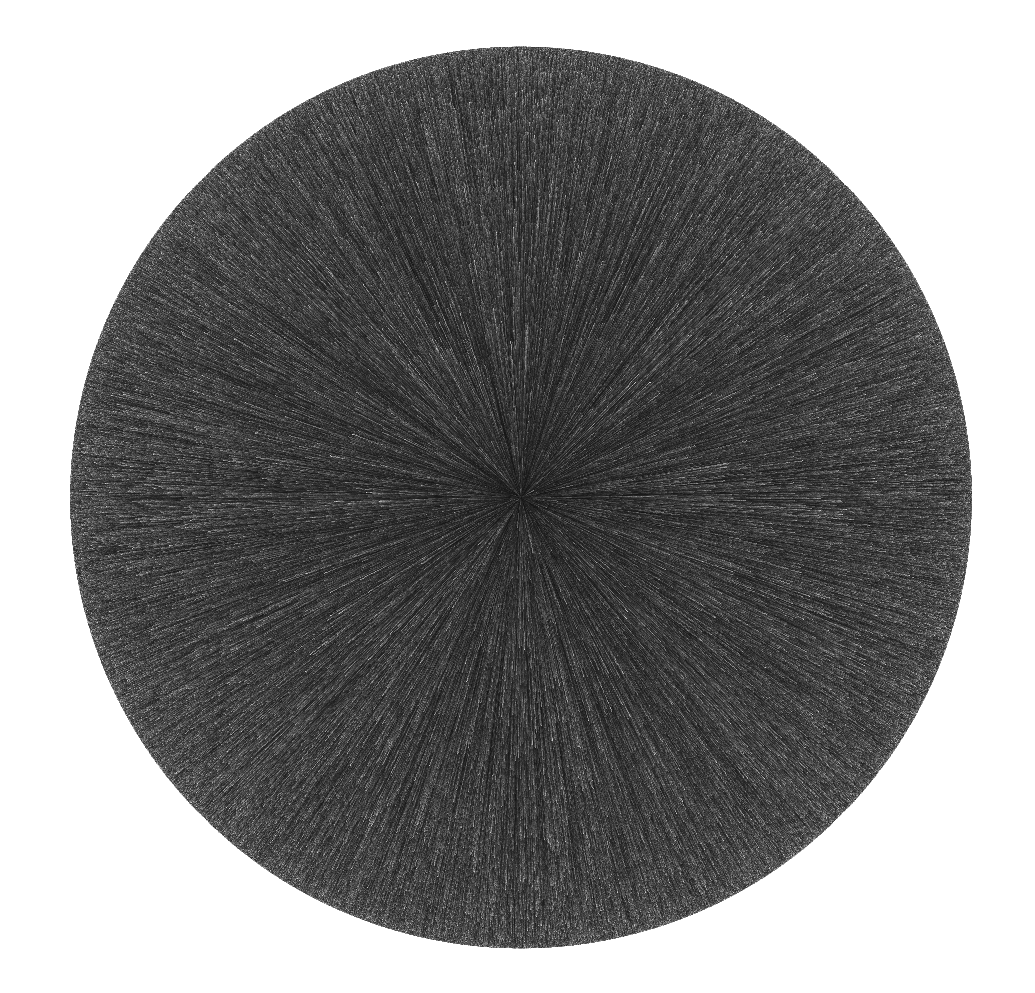
\includegraphics[width = 3 in]{3.png}
  \caption{
Where $D = 3$.
The normals are isotropic.
}
\end{figure}

\begin{figure} 
\centering
\label{fig3}
  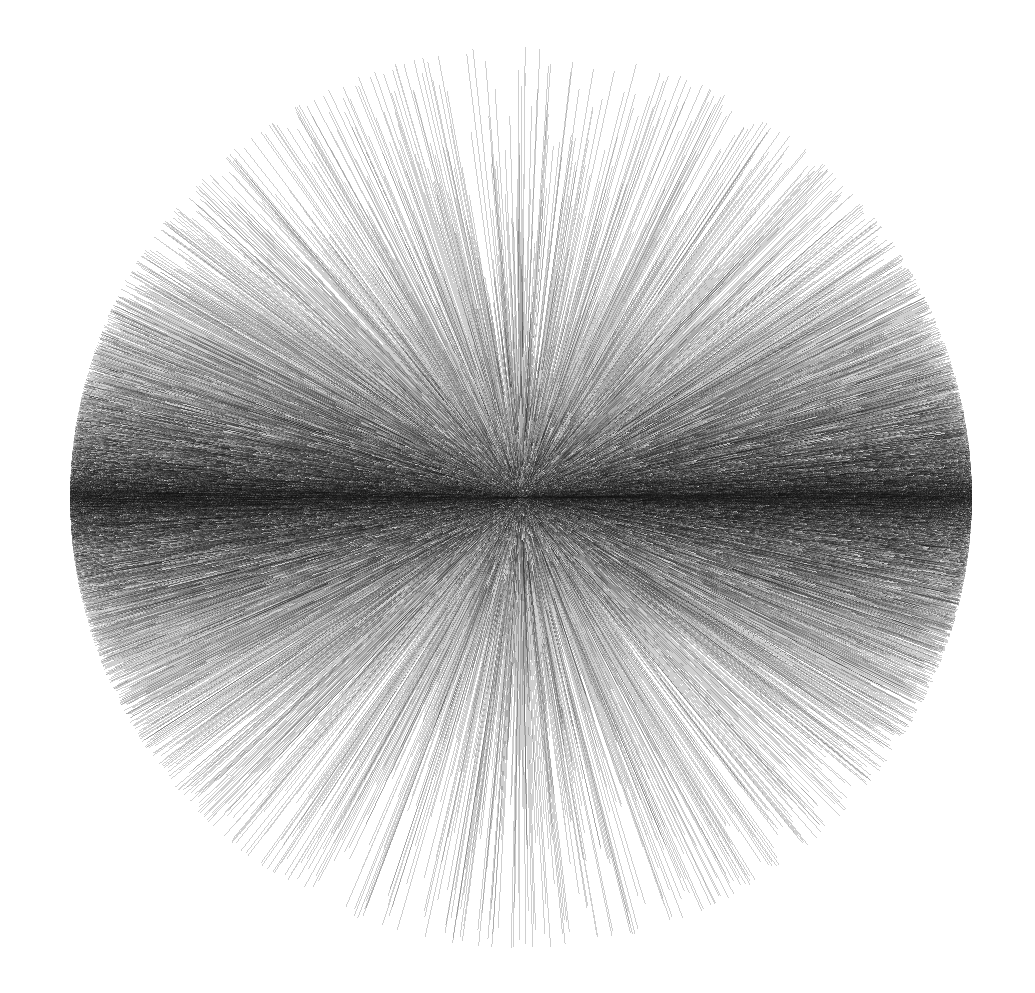
\includegraphics[width = 3 in]{2.1.png}
  \caption{
Where $D = 2.1$.
The normals are increasingly anisotropic.
}
\end{figure}

\begin{figure} 
\centering
\label{fig4}
  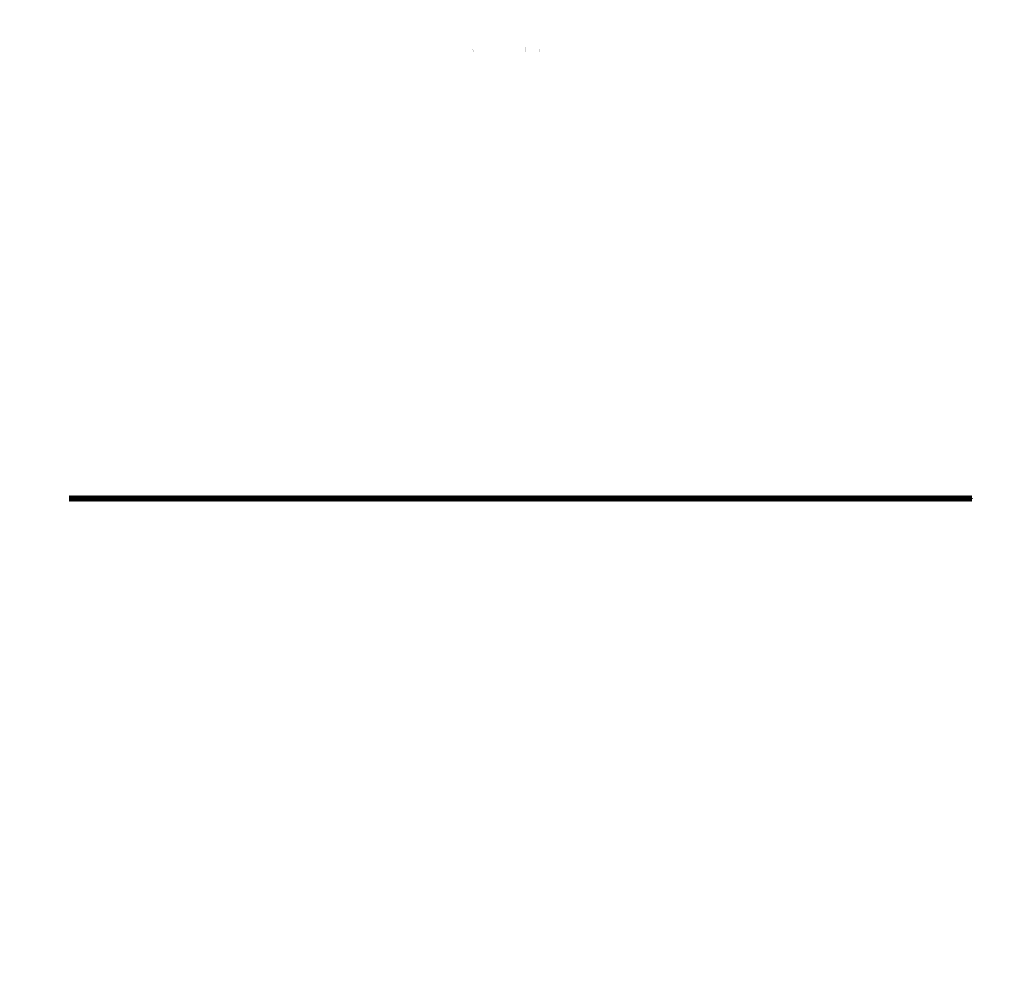
\includegraphics[width = 3 in]{2.001.png}
  \caption{
Where $D = 2.001$.
The normals are anisotropic.
}
\end{figure}





\end{document}









